\documentclass[letterpaper,12pt]{article}
\usepackage{array}
\usepackage{geometry}
\geometry{letterpaper,tmargin=1in,bmargin=1in,lmargin=1.25in,rmargin=1.25in}
%\renewcommand\headrulewidth{0pt}
%\renewcommand\footrulewidth{0pt}
\usepackage{amsmath}
\usepackage{amssymb}
\usepackage{amsthm}
\usepackage{enumerate}
%\usepackage{harvard}
%\usepackage{setspace}
\usepackage{float,color}
\usepackage[pdftex]{graphicx}
\usepackage{hyperref}
\hypersetup{colorlinks,linkcolor=red,urlcolor=blue}
\theoremstyle{definition}
\newtheorem{theorem}{Theorem}
\newtheorem{acknowledgement}[theorem]{Acknowledgement}
\newtheorem{algorithm}[theorem]{Algorithm}
\newtheorem{axiom}[theorem]{Axiom}
\newtheorem{case}[theorem]{Case}
\newtheorem{claim}[theorem]{Claim}
\newtheorem{conclusion}[theorem]{Conclusion}
\newtheorem{condition}[theorem]{Condition}
\newtheorem{conjecture}[theorem]{Conjecture}
\newtheorem{corollary}[theorem]{Corollary}
\newtheorem{criterion}[theorem]{Criterion}
\newtheorem{definition}[theorem]{Definition}
\newtheorem{derivation}{Derivation} % Number derivations on their own
\newtheorem{example}[theorem]{Example}
\newtheorem{exercise}[theorem]{Exercise}
\newtheorem{lemma}[theorem]{Lemma}
\newtheorem{notation}[theorem]{Notation}
\newtheorem{problem}[theorem]{Problem}
\newtheorem{proposition}{Proposition} % Number propositions on their own
\newtheorem{remark}[theorem]{Remark}
\newtheorem{solution}[theorem]{Solution}
\newtheorem{summary}[theorem]{Summary}
%\numberwithin{equation}{section}
\bibliographystyle{aer}
\newcommand\ve{\varepsilon}
\newcommand\boldline{\arrayrulewidth{1pt}\hline}


\begin{document}

\begin{flushleft}
   \textbf{\large{Problem Set \#3}} \\
   MACS 40000, Dr. Evans \\
   Alexandre Sollaci
\end{flushleft}

\vspace{5mm}

\noindent\begin{enumerate}
   \item \textbf{Checking Feasibility in the steady state}
   
   In this question, I have coded up the \texttt{b\_cnstr} object as follows: \texttt{b\_cnstr[0] = c\_cnstr[0]}. Furthermore, if \texttt{s > 0} and \texttt{c\_cnstr[s] == True}, then \texttt{b\_cnstr[s] == True} and \texttt{b\_cnstr[s+1] == True}.
	\begin{enumerate}[(a)]
		\item If \texttt{bvec\_guess = np.ones(S-1)}, the \texttt{feasible()} function output is
		
		\begin{verbatim}
b_cnstr = array([
       True, False, False, False, False, False, False, False, False,
       False, False, False, False, False, False, False, False, False,
       False, False, False, False, False, False, False, False, False,
       False, False, False, False, False, False, False, False, False,
       False, False, False, False, False, False, False, False, False,
       False, False, False, False, False, False, False, False, False,
       False, False, False, False, False, False, False, False, False,
       False, False, False, False, False, False, False, False, False,
       False, False, False, False, False, False, False], dtype=bool),
c_cnstr = array([ 
       True, False, False, False, False, False, False, False, False,
       False, False, False, False, False, False, False, False, False,
       False, False, False, False, False, False, False, False, False,
       False, False, False, False, False, False, False, False, False,
       False, False, False, False, False, False, False, False, False,
       False, False, False, False, False, False, False, False, False,
       False, False, False, False, False, False, False, False, False,
       False, False, False, False, False, False, False, False, False,
       False, False, False, False, False, False, False, False], dtype=bool),
K_cnstr = False
		\end{verbatim}
		The first constraint is violated as savings are too high.
		
		\item The \texttt{feasible()} function output is
		
		\begin{verbatim}
b_cnstr = array([
       False, False, False, False, False, False, False, False, False,
       False, False, False, False, False, False, False, False, False,
       False, False, False, False, False, False, False, False, False,
       False, False, False, False, False, False, False, False, False,
       False, False, False, False, False, False, False, False, False,
       False, False, False, False, False, False, False, False, False,
       False, False, False,  True,  True, False, False, False, False,
       False, False,  True,  True, False, False, False, False, False,
       False,  True,  True, False, False, False, False], dtype=bool),
c_cnstr = array([
       False, False, False, False, False, False, False, False, False,
       False, False, False, False, False, False, False, False, False,
       False, False, False, False, False, False, False, False, False,
       False, False, False, False, False, False, False, False, False,
       False, False, False, False, False, False, False, False, False,
       False, False, False, False, False, False, False, False, False,
       False, False, False,  True, False, False, False, False, False,
       False, False,  True, False, False, False, False, False, False,
       False,  True, False, False, False, False, False, False], dtype=bool),
K_cnstr = False
		\end{verbatim}				
		Consumption is violated in the following entries: 
		\begin{verbatim}
		np.where(c_cnstr == True)
 (array([57, 65, 73], dtype=int64),)
		\end{verbatim}
		Those entries combine two features. First, this is where the labor supply drops to 0.2; second, it immediately follows a period when savings are negative.
		
		\item Once again, the \texttt{feasible()} function output is
		
		\begin{verbatim}
b_cnstr = array([
       False, False, False, False, False, False, False, False, False,
       False, False, False, False, False, False, False, False, False,
       False, False, False, False, False, False, False, False, False,
       False, False, False, False, False, False, False, False, False,
       False, False, False, False, False, False, False, False, False,
       False, False, False, False, False, False, False, False, False,
       False, False, False, False, False, False, False, False, False,
       False, False, False, False, False, False, False, False, False,
       False, False, False, False, False, False, False], dtype=bool), 
c_cnstr = array([
       False, False, False, False, False, False, False, False, False,
       False, False, False, False, False, False, False, False, False,
       False, False, False, False, False, False, False, False, False,
       False, False, False, False, False, False, False, False, False,
       False, False, False, False, False, False, False, False, False,
       False, False, False, False, False, False, False, False, False,
       False, False, False, False, False, False, False, False, False,
       False, False, False, False, False, False, False, False, False,
       False, False, False, False, False, False, False, False], dtype=bool),
K_cnstr = False
		\end{verbatim}
		In this case, the constraints are never violated.
		
		\item To guarantee that the initial guess is feasible, we should choose savings that are not ``too high" -- so somewhat close to zero -- and that do not become negative when the agent is close to having the exogenous decrease in his labor supply.
	\end{enumerate}

\item \textbf{Solve for the steady state equilibrium.}	  
	
	\begin{enumerate}[(a)]
	\item The \texttt{get\_SS} function returns
	\begin{verbatim}
	{'C_ss': 98.895859560202624,
 'EulErr_ss': array([  
          4.68514116e-14,  -2.44249065e-15,  -4.49640325e-14,
          5.77315973e-15,   2.22044605e-16,  -6.66133815e-16,
          4.44089210e-16,   4.44089210e-16,  -7.77156117e-16,
          1.11022302e-15,  -5.55111512e-16,   6.66133815e-16,
         -2.22044605e-16,   2.22044605e-16,  -1.55431223e-15,
          1.55431223e-15,  -1.11022302e-15,   2.22044605e-16,
         -2.22044605e-16,  -3.33066907e-16,  -2.22044605e-16,
          1.77635684e-15,  -6.66133815e-16,   1.77635684e-15,
         -2.66453526e-15,  -1.88737914e-15,   1.11022302e-15,
          1.33226763e-15,   6.66133815e-16,  -1.33226763e-15,
          1.11022302e-15,  -8.88178420e-16,   8.88178420e-16,
         -1.99840144e-15,   0.00000000e+00,  -1.66533454e-15,
          8.21565038e-15,  -6.77236045e-15,   8.88178420e-16,
          4.66293670e-15,  -5.44009282e-15,   7.10542736e-15,
          2.22044605e-16,  -5.32907052e-15,   4.88498131e-15,
          0.00000000e+00,  -1.77635684e-15,  -4.88498131e-15,
          5.32907052e-15,  -5.55111512e-16,  -8.32667268e-15,
          1.02140518e-14,   5.99520433e-15,  -4.14113188e-14,
          3.17523785e-14,  -4.88498131e-15,   5.10702591e-15,
         -3.06421555e-14,   4.26325641e-14,   6.32827124e-14,
         -2.62012634e-14,  -5.52891066e-14,  -4.81836793e-14,
         -1.39888101e-14,   1.19904087e-14,   3.59712260e-14,
          5.28466160e-14,   3.75255382e-14,  -7.77156117e-16,
         -5.81756865e-14,  -4.15223411e-14,   2.10942375e-14,
          6.66133815e-15,  -6.66133815e-16,   4.44089210e-16,
          3.33066907e-15,  -1.55431223e-15,   1.06581410e-14,
         -1.12132525e-14]),
 'K_ss': 501.94151215269738,
 'RCerr_ss': 9.2370555648813024e-14,
 'Y_ss': 123.99293516783759,
 'b_ss': array([  
          0.06051915,   0.12544728,   0.19494146,   0.26916448,
          0.3482851 ,   0.43247822,   0.52192513,   0.61681373,
          0.71733879,   0.82370217,   0.93611311,   1.05478847,
          1.17995304,   1.3118398 ,   1.45069023,   1.59675463,
          1.75029242,   1.91157249,   2.08087354,   2.25848443,
          2.44470458,   2.6398443 ,   2.84422524,   3.05818079,
          3.28205648,   3.51621046,   3.76101392,   4.01685163,
          4.28412237,   4.56323945,   4.85463128,   5.15874189,
          5.4760315 ,   5.80697711,   6.15207313,   6.511832  ,
          6.88678483,   7.27748213,   7.68449447,   8.10841322,
          8.54985132,   9.00944409,   9.48784999,   9.9857515 ,
         10.50385598,  11.04289661,  11.60363329,  12.18685362,
         12.79337396,  13.42404039,  14.07972987,  14.76135135,
         15.46984691,  15.10214629,  14.72305542,  14.33215564,
         13.92901307,  13.51317797,  13.08418424,  12.64154879,
         12.18477091,  11.71333163,  11.2266931 ,  10.72429784,
         10.20556806,   9.66990489,   9.11668766,   8.54527306,
          7.95499433,   7.34516041,   6.71505505,   6.06393589,
          5.39103352,   4.69555046,   3.97666018,   3.23350602,
          2.46520007,   1.67082209,   0.84941826]),
 'c_ss': array([ 
         1.3195392 ,  1.31733671,  1.31513791,  1.31294277,  1.31075129,
         1.30856348,  1.30637931,  1.30419879,  1.30202191,  1.29984866,
         1.29767905,  1.29551305,  1.29335067,  1.29119189,  1.28903672,
         1.28688515,  1.28473717,  1.28259277,  1.28045196,  1.27831472,
         1.27618104,  1.27405092,  1.27192437,  1.26980136,  1.26768189,
         1.26556596,  1.26345357,  1.26134469,  1.25923934,  1.25713751,
         1.25503918,  1.25294435,  1.25085302,  1.24876519,  1.24668083,
         1.24459996,  1.24252256,  1.24044862,  1.23837815,  1.23631113,
         1.23424757,  1.23218744,  1.23013076,  1.22807751,  1.22602769,
         1.22398129,  1.2219383 ,  1.21989872,  1.21786255,  1.21582978,
         1.2138004 ,  1.2117744 ,  1.20975179,  1.20773256,  1.20571669,
         1.20370419,  1.20169505,  1.19968926,  1.19768682,  1.19568773,
         1.19369197,  1.19169954,  1.18971043,  1.18772465,  1.18574218,
         1.18376302,  1.18178716,  1.17981461,  1.17784534,  1.17587936,
         1.17391666,  1.17195724,  1.17000109,  1.1680482 ,  1.16609858,
         1.1641522 ,  1.16220908,  1.1602692 ,  1.15833256,  1.15639915]),
 'r_ss': 0.036459330934041259,
 'ss_time': 0.06646503229785594,
 'w_ss': 1.3800583537516151}
	\end{verbatim}
	
	\item The steady state distribution of consumption and savings can be seen in figure 1.
	
	
	\item A few things happen:
	\begin{itemize}
	\item First, the fact that consumers ``retire" earlier means that their total time endowment decreased. This acts as a negative income shock, decreasing total consumption.
	\item It also increases the relative endowment inequality between the old and the young, making it harder for consumers to smooth their consumption. For this reason, consumption when young increases while consumption when old decreases.
	\item Once again because of the higher relative endowment inequality between the young and the old, consumers will save more to increase their consumption when old. This increases the capital supply, decreasing the marginal product of capital and thus the interest rate.
	\item The increase in the supply of capital also increases the marginal product of labor. In addition, the lower supply of labor further increases the marginal product of labor, meaning that the wage increases.
	\item Finally, consumers will save more ``aggressively" in order to smooth their consumption. This shifts the peak of savings both up and and to an earlier age. 
	\end{itemize}
The new steady state is described by the following output and figure 2 below.

\begin{verbatim}
{'C_ss': 86.383344908512726,
 'EulErr_ss': array([  
          4.44089210e-16,  -3.33066907e-16,  -4.44089210e-16,
         -1.11022302e-15,   8.88178420e-16,   0.00000000e+00,
          0.00000000e+00,   0.00000000e+00,  -9.99200722e-16,
          6.66133815e-16,   0.00000000e+00,  -5.55111512e-16,
         -3.33066907e-16,   2.44249065e-15,  -2.77555756e-15,
          8.88178420e-16,  -6.66133815e-16,   4.44089210e-16,
          1.55431223e-15,  -2.22044605e-16,   6.66133815e-16,
          1.55431223e-15,  -5.66213743e-15,  -7.77156117e-16,
          9.10382880e-15,  -7.10542736e-15,   2.88657986e-15,
          1.77635684e-15,  -3.33066907e-16,  -4.44089210e-15,
          4.44089210e-15,  -6.21724894e-15,   1.06581410e-14,
         -5.77315973e-15,  -2.22044605e-15,   7.32747196e-15,
         -1.06581410e-14,  -6.32827124e-15,   1.70974346e-14,
         -3.10862447e-15,   9.10382880e-15,  -1.07691633e-14,
         -2.77555756e-15,   2.88657986e-15,  -2.22044605e-16,
         -1.50990331e-14,   2.68673972e-14,   2.22044605e-15,
         -1.93178806e-14,  -7.99360578e-15,   1.02140518e-14,
         -3.66373598e-15,   7.54951657e-15,   2.22044605e-16,
         -2.22044605e-16,  -5.66213743e-15,   4.21884749e-15,
         -3.66373598e-15,   2.66453526e-15,  -5.32907052e-15,
          3.99680289e-15,  -4.44089210e-16,   2.22044605e-16,
         -1.33226763e-15,  -4.10782519e-15,   3.99680289e-15,
          2.22044605e-16,  -1.55431223e-15,   6.66133815e-16,
          4.44089210e-16,  -9.99200722e-16,   1.11022302e-15,
         -5.55111512e-16,  -1.11022302e-16,   1.11022302e-15,
         -1.88737914e-15,  -1.55431223e-15,   1.55431223e-15,
         -4.44089210e-16]),
 'K_ss': 611.27200934683106,
 'RCerr_ss': 2.1671553440683056e-13,
 'Y_ss': 116.9469453758545,
 'b_ss': array([ 
          0.12750186,   0.26877057,   0.42394716,   0.59317577,
          0.77660375,   0.97438164,   1.18666326,   1.41360578,
          1.65536971,   1.91211899,   2.18402106,   2.47124688,
          2.77397097,   3.09237154,   3.42663045,   3.77693334,
          4.14346965,   4.52643272,   4.92601977,   5.34243208,
          5.77587492,   6.22655773,   6.69469412,   7.18050193,
          7.68420335,   8.20602495,   8.74619773,   9.30495725,
          9.88254364,  10.47920172,  11.09518106,  11.73073603,
         12.38612593,  13.06161499,  13.75747256,  14.47397307,
         15.2113962 ,  15.97002694,  16.75015566,  17.55207821,
         17.10917075,  16.66717719,  16.22604588,  15.78572483,
         15.3461617 ,  14.9073038 ,  14.46909804,  14.03149098,
         13.59442876,  13.15785715,  12.72172146,  12.28596662,
         11.8505371 ,  11.41537693,  10.98042966,  10.54563841,
         10.11094578,   9.67629388,   9.24162434,   8.80687824,
          8.37199615,   7.93691806,   7.50158346,   7.06593121,
          6.62989962,   6.1934264 ,   5.75644864,   5.3189028 ,
          4.88072472,   4.44184957,   4.00221184,   3.56174537,
          3.12038329,   2.67805799,   2.23470117,   1.79024375,
          1.34461593,   0.89774709,   0.44956585]),
 'c_ss': array([ 
         1.45615469,  1.44455041,  1.4330386 ,  1.42161854,  1.41028948,
         1.3990507 ,  1.38790149,  1.37684112,  1.3658689 ,  1.35498412,
         1.34418607,  1.33347408,  1.32284746,  1.31230552,  1.30184759,
         1.291473  ,  1.28118109,  1.27097119,  1.26084266,  1.25079484,
         1.2408271 ,  1.23093879,  1.22112928,  1.21139795,  1.20174416,
         1.19216731,  1.18266677,  1.17324195,  1.16389224,  1.15461703,
         1.14541574,  1.13628778,  1.12723255,  1.11824949,  1.10933802,
         1.10049757,  1.09172756,  1.08302744,  1.07439666,  1.06583466,
         1.05734088,  1.0489148 ,  1.04055586,  1.03226354,  1.0240373 ,
         1.01587662,  1.00778097,  0.99974983,  0.9917827 ,  0.98387905,
         0.9760384 ,  0.96826022,  0.96054403,  0.95288933,  0.94529564,
         0.93776246,  0.93028931,  0.92287571,  0.9155212 ,  0.90822529,
         0.90098753,  0.89380745,  0.88668458,  0.87961848,  0.87260869,
         0.86565476,  0.85875624,  0.8519127 ,  0.8451237 ,  0.8383888 ,
         0.83170758,  0.82507959,  0.81850443,  0.81198166,  0.80551088,
         0.79909166,  0.79272359,  0.78640628,  0.78013931,  0.77392228]),
 'r_ss': 0.016961075029897021,
 'ss_time': 0.07017229105258593,
 'w_ss': 1.5836565519646923}
\end{verbatim}

	\end{enumerate}
	
\end{enumerate}
\clearpage

\section*{Figures}

\begin{figure}[h!]
	\centering
	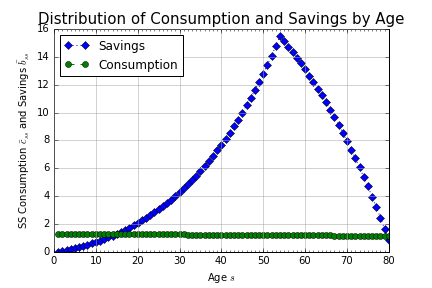
\includegraphics[scale=.8]{code/images/cons_savings_dist}
	\caption{Distribution of consumption and savings in steady state.}
	\end{figure}
	
	\begin{figure}[h!]
	\centering
	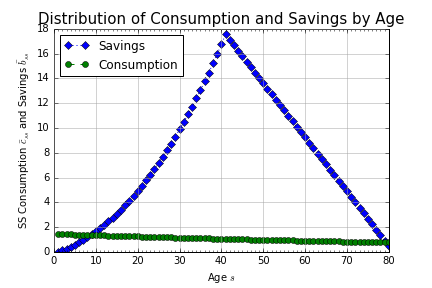
\includegraphics[scale=.8]{code/images/cons_savings_dist2}
	\caption{Distribution of consumption and savings in steady state with ``new" labor supply.}
	\end{figure}

\end{document}





